\chapter{Úvod}
Some introductory text\dots

\section{Aplikace DDA}
Algoritmy vyvažování obtížnosti lze využít v širokém spektru aplikací. Mohou být vhodné všude tam, kde je vyžadována určitá dovednost, schopnost. V takovém případě může být obtížné aplikaci, program navrhnout tak, aby byl dobře využitelný velkým spektrem lidí různých schopností.

DDA můžeme nalézt nejen v zábavním průmyslu, ale i u vážných her. Adaptivní obtížnost programu může zefektivňovat léčbu nemocných lidí, nahrazovat osobního trenéra či učitele. V následujících 4 podkapitolách popisuji konkrétní užití dynamické obtížnosti v komerční i v akademické sféře.

\subsection{Zábavní průmysl}

Hráče počítačových her lze rozdělit dle jejich schopností od příležitostných až po hardcore hráče. Většina her obsahuje statickou volbu obtížnosti na začátku hry. V některých případech to nemusí být dostačující, a proto se tvůrci komerčních her snaží více, či méně úspěšně implementovat adaptivní obtížnost.
Na stránce \cite{1} lze nalézt desítky příkladů všech různých žánrů. Do následujícího seznamu 5 her jsem vybral ty známější příklady.


\subsubsection{Left 4 Dead}
\label{sec:Left4Dead}

V zombie hře Left 4 Dead pojmenovali adaptivní systém The AI Director. Na základě aktuálního hráčova zdraví, munice a relativní pozice v rámci dané úrovně hry The AI Director generuje ve hře zbraně, munici, lékárničky na pomoc hráči a naopak generuje lehčí, či těžší nepřátele. Např. blíží-li se hráč konci úrovně a má plné zdraví i munici, hra vygeneruje těžkého soupeře „Tank“. \cite{2}

\subsubsection{Max Payne 3}

Hra Max Payne 3 obsahuje celkem 5 statických obtížností(Easy, Medium, Hard, Hardcore, Old School), které se v průběhu hry adaptivně přizpůsobují hráči. Čím nižší obtížnost si hráč na začátku zvolí, tím více se hra může měnit ve prospěch hráče.
Jestliže hráč opakovaně umírá, dostane se mu pomoci ve formě bonusových léků(painkillers), které umožní lehčí projití daného úseku hry. Při smrti na lehkou a střední obtížnost se hráčův avatar obnoví minimálně s jedním plným zásobníkem pro každou zbraň vyjma granátometů. Plus za každé tři úmrtí ve stejném úseku dostane jeden painkiller navíc až do maximálního limitu devíti painkillerů.
Na těžkou obtížnost je dynamická obtížnost více limitovaná. Jestliže hráč zemře 5 krát po sobě, dostane jeden painkiller. Pokud zemře podesáté, dostane druhý painkiller. Další léky mu hra již nepřidává. \cite{3}

\subsubsection{The Elder Scrolls IV: Oblivion}

Dalším příkladem mohou být hry Oblivion a Fallout 3 od Bethesda Softworks. V Oblivionu nepřátelé levelují s hráčem. Stráže ve městě mají level o 2-5 vyšší než vy, banditi mají level o 2-5 nižší atd. Tímto je docíleno, že se můžete vydat kamkoli ve hře aniž byste narazili na příliš obtížné nepřátele. Mimo síly nepřátel se adaptivně upravuje druh nepřátel, jejich vybavení, nabízení zboží v obchodech apod. Občas může docházet k nelogickým situacím, kdy obyčejní potulní bandité mají na sobě nejmodernější brnění, nebo kdy máte za úkol donést vlčí kožešinu ve světe, kde už tak slabí nepřátelé se nepohybují. \cite{4}

\subsubsection{Mario Kart Wii}

Závodní simulátory jsou dobře známé využíváním adaptivní obtížnosti her a mezi nejznámější zástupce patří arkádové závody Mario Kart. Ve hře se adaptivně mění rychlost protivníků a také bonusové power-upy, které můžete sbírat. Hra podporuje natolik prohrávající hráče, že ať už je aktuální stav hry jakýkoli, může vyhrát kdokoliv.
Což lze brát jako velkou výhodu, kdy žádný z hráčů nemá důvod ke vzdávání hry. Nevýhodou je právě známost a odhalení tohoto systému, a tudíž je lehce zneužitelná. Např. konkrétně ve variantě Mario Kart Wii je vedoucí hráč na začátku posledního kola bombardován modrým krunýřem, či jinou devastující zbraní a je záhy poslán na poslední místo. Nejlepší strategií je projet do posledního kola na druhé pozici, což moc nedává smysl. \cite{5}

\subsubsection{Pro Evolution Soccer 2008}

Úspěšný fotbalový simulátor Pro Evolution Soccer se ve své verzi s číslem 2008 chlubil adaptivním systémem nazvaný Teamvision. Teamvision se učí od hráče jeho styl hry a snaží se upravovat taktiku svého týmu, aby co nejlépe reagovala na tu soupeřovu. Použití jedné finty může fungovat jednou, dvakrát, ale později již naprosto stejná finta nevede k vítězství. \cite{6}

\subsection{Cvičení}

Herní zařízení jako jsou Microsoft Kinect a Nintendo Wii dávají prostor pohybovým hrám. Stejně jako v jiných příkladech i zde platí, že existují lidé s diametrálně odlišnou fyzickou kondicí. Kondice se v ideálním případě při opakované hře stále zlepšuje, a proto je vhodné k tomu přizpůsobovat obtížnost hry.
Příkladem takové aplikace může být jednoduchá chodící hra hratelná v internetovém prohlížeči, jež má za úkol motivovat starší lidi k pohybu.
V druhém případě nebylo využito žádné ze zmíněných zařízení. Autoři článku \cite{7} se zaměřili na jogging v páru. 

\subsubsection{Podpora pohybu starších lidí}

Evropská populace stárne a odmítání pohybu staršími lidmi se stává závažným problémem. Z nedostatku fyzické námahy klesá síla a ohebnost těchto lidí, ztrácejí kostní hmotu a tím zvyšují pravděpodobnost pádu a zlomení některé z končetin. Z tohoto důvodu se skupina z Technologického institutu zaměřila na vývoj hry, jež má starší lidi motivovat k pohybu a jejíž nedílnou součástí je vyvažování obtížnosti. \cite{8}
Hra je vytvářena v HTML5 pro běžné použití ve webových prohlížečích a využívá Microsoft Kinect ovládání.
Základním cílem hry je udělat předem dané množství kroků v každé hře. Kroky jsou zaznamenávány pomocí Kinectu. Hráč musí jít v rytmu a zároveň se musí vyhýbat dírám v zemi. V případě špatných, či propásnutých kroků hráčův avatar zpomalí.
Při hře více hráčů se všichni zúčastnění snaží jít ve stejném tempu. Obtížnost je upravována přidáváním, či odebíráním překážek pro jednotlivé hráče a tím je motivuje k opakovanému hraní.

\begin{figure}
  \centering
  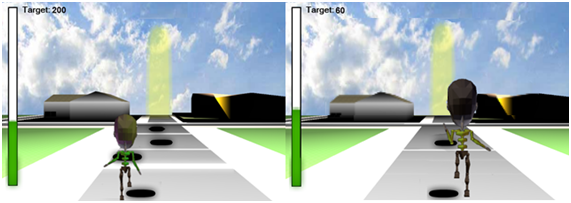
\includegraphics{ch1elderlypeople}
	\caption{Screenshoty HTML5 hry. Vlevo hraje nadaný hráč, vpravo s menší dovedností. \cite{8} }
	\label{ch1elderlypeople}
\end{figure}

\subsubsection{Jogging na dálku}

Ne každého baví běhat po parku samostatně a zároveň může být těžké najít někoho, kdo by si s vámi zaběhal ve stejnou dobu. Řešením může být jogging na dálku (jogging over distance), kdy dva lidé běží ve stejnou dobu, ale každý běží jinde, třeba i v jiném státě. Oba cvičící se dorozumívají přes telefon se sluchátky na hlavě. Povídají si, navzájem se podporují.
Různí lidé mají různou fyzickou kondici a může být problém se navzájem přizpůsobit v běhu tak, aby oba dva jedinci byli přibližně stejně namáhání. Neměla by nastat situace, kdy jeden udýchaně nemůže skoro mluvit a druhému naopak cvičení nic nedává.
V článku Balancing Exertion Experiences \cite{7} popisují svůj přístup k dané problematice. Každý z joggujících partnerů má při sobě chytrý telefon a měřič srdeční frekvence. Na telefonu mají nastavenou svojí ideální, cílovou srdeční frekvenci každý dle své fyzické kondice, případně dle doporučení doktora. Jestliže oba partneři mají srdeční frekvenci relativně stejnou vůči své cílové, pak je vše v pořádku. Partneři mohou běžet několik minut s cílovou srdeční frekvencí, poté se vyhecují, že na chvíli zrychlí a běží např. na 120\% své cílové frekvence. Pokud nastane situace, kdy první partner běží na 80\%, druhý na 110\%, jak vhodně donutit prvního zrychlit a druhého zpomalit? 

Autoři článku přišli se zajímavým řešením. Pomocí sluchátek mohou simulovat vjem, kdy se partneři slyší vedle sebe, kdy jeden slyší druhého před sebou, případně za sebou. Ve výše uvedeném příkladu by partner běžící na 110\% slyšel spoluběžce za ním, což by ho donutilo zpomalit. Opačně partner běžící na 80\% by slyšel toho druhého před sebou a byl by donucen zrychlit, aby se ve výsledku slyšeli co nejlépe, vedle sebe.



\endinput
%%
%% End of file `ch01.tex'.
